\documentclass[12pt]{spieman}  % 12pt font required by SPIE;
%\documentclass[a4paper,12pt]{spieman}  % use this instead for A4 paper
\usepackage{amsmath,amsfonts,amssymb}
\usepackage{graphicx}
\usepackage{setspace}
\usepackage{tocloft}
\usepackage{booktabs}
\usepackage{lineno}

\title{Consistency ordinary differential equations network for person re-identification}

\author[a]{Yin Huang}
\author[b,c,*]{Jieyu Ding}
\affil[a]{Qingdao University, School of Computer Science and Technology, Qingdao, China, 266071}
\affil[b]{Qingdao University, School of Mathematics and Statistics, Qingdao, China, 266071}
\affil[c]{Qingdao University, Center for Computational Mechanics and Engineering Simulation, Qingdao, China, 266071}

\renewcommand{\cftdotsep}{\cftnodots}
\cftpagenumbersoff{figure}
\cftpagenumbersoff{table}
\begin{document}
	\maketitle
	\linenumbers
	
	\begin{abstract}
		Person re-identification (Re-ID) aims to retrieve images of a given individual across different camera views. When images contain substantial identity-irrelevant information, the discriminability of person features degrades, leading to reduced recognition accuracy or even failure to recognize individuals. To address this issue, a novel consistency ordinary differential equations network (CODEN) is proposed, utilizing a dynamical system and incorporating a consistency regularization loss for Re-ID. Specifically, CODEN primarily consists of two key modules: the dynamic feature extraction (DFE) module and the stable trajectory evolution (STE) module. The DFE module parameterizes ordinary differential equations to model the dynamical system and dynamically extracts global saliency information by solving these equations using numerical integrators. The STE module perturbs the initial value of the dynamical system and employs a consistency regularization loss to learn robust feature representations, resisting interference from identity-irrelevant information. Experiments are conducted on three datasets, including Market-1501, DukeMTMC-reID, and CUHK03. The experimental results demonstrate the effectiveness of CODEN in enhancing person Re-ID performance.
	\end{abstract}
	
	% Include a list of up to six keywords after the abstract
	\keywords{person re-identification, dynamical system, ordinary differential equation, consistency regularization loss}
	
	% Include email contact information for corresponding author
	{\noindent \footnotesize\textbf{*}Jieyu Ding,  \linkable{djy@qdu.edu.cn} }
	
	\begin{spacing}{2}   % use double spacing for rest of manuscript
		
		\section{Introduction}
		\label{sect:intro}  % \label{} allows reference to this section
		Person re-identification (Re-ID) aims to match individual images captured from non-overlapping camera views \cite{nambiar2019gait}. Re-ID technology, to a certain extent, overcomes the inefficiency of manual retrieval and compensates for the visual limitations of current fixed cameras. It has gradually become one of the research hotspots in the fields of computer vision and pattern recognition due to its wide range of applications, including surveillance and criminal investigations \cite{zhang2024joint,wang2023multi,hu2024pose}.
		
		Existing person Re-ID methods based on deep learning can be roughly categorized into global-based methods, local-based methods, and cues-based methods. Global-based methods primarily rely on neural networks to extract features that capture the overall appearance of a pedestrian \cite{luo2019bag, ghorbel2022masking}. Local-based methods typically use grid segmentation, dividing the pedestrian image into several blocks and extracting features from different regions for identification \cite{sun2018beyond, zhang2021appearance}. Cues-based methods utilize external visual cues, such as pose landmarks \cite{miao2019pose} and semantic parsing \cite{guo2019beyond}, to detect key pedestrian regions. These works improve the performance of Re-ID to some extent. However, pedestrian images often include interference from identity-irrelevant factors, such as foreground occlusions and background clutter, which increases the difficulty of discriminative representation learning for Re-ID in realistic scenarios.
		
		Adversarial defense strategies are techniques designed to protect neural networks from noise perturbations \cite{szegedy2013intriguing, wang2020transferable, wang2022occluded}. Some methods treat identity-irrelevant information in images as adversarial attacks and employ defensive strategies to protect Re-ID models from such perturbations. For instance, Zhao et al. \cite{zhao2021incremental} progressively generate adversarial examples and use an occlusion suppression strategy to enhance the representation of features in visible body regions. Similarly, Dong et al. \cite{dong2023erasing} perturb feature maps to create multiple adversarial representations and utilize generative adversarial networks to learn robust pedestrian features. However, these methods primarily rely on random rectangular perturbation strategies to generate adversarial representations, often overlooking the relationship between the perturbed features and the discriminative information. For example, due to the irregular shape of pedestrians, randomly perturbing regions may disrupt key features such as clothing, arms, face, legs, and body shape, which are highly discriminative. This can introduce ambiguity in certain situations, ultimately impairing recognition performance.
		
		In this paper, we propose a consistency ordinary differential equations network (CODEN), which leverages a dynamical system enhanced by consistency regularization loss for Re-ID.
		\textcolor{yellow}{Specifically, CODEN integrates a continuous dynamical system governed by ordinary differential equations (ODEs) into feature extraction, thereby capturing pedestrian saliency information. In addition, CODEN utilizes the system's trajectory to generate perturbations in the feature space.}
		Furthermore, it employs a consistency regularization loss to prevent the network from focusing on undesirable information and to avoid confusing the learning dynamical system.

		The main contributions of this paper can be summarized as follows:
		
		\begin{itemize}
			\item We propose CODEN, a dynamical system enhanced by consistency regularization loss for Re-ID, which mitigates the impact of identity-irrelevant information interference.
			\item \textcolor{yellow}{We propose a consistency regularization loss to learn identification features more effectively.}
			\item Extensive experiments on the Market-1501, DukeMTMC-reID, and CUHK03 datasets demonstrate the superiority of CODEN.
		\end{itemize}
		
		The remainder of this paper is organized as follows: The related works are introduced in Section \ref{section:related_work}; The details of the proposed method are elaborated in Section \ref{section:proposed_method}; The experimental comparison and analysis are reflected in Section \ref{section:experiment}; The conclusion of the present paper is summarized in Section \ref{section:conclusion}.
		
		\section{Related work} \label{section:related_work}
		\subsection{Person re-identification}
		\textcolor{yellow}{According to the feature learning technologies, person re-ID methods can be roughly categorized into hand-crafted feature-based methods and deep learning-based methods. Hand-crafted feature-based methods focus on manually designing features, which includes both feature extraction\cite{lowe2004distinctive, ojala2002multiresolution,dalal2005histograms} and metric learning\cite{pedagadi2013local,liao2015person,tao2016person}. }
		
		\textcolor{yellow}{Deep learning-based methods primarily employ data-driven approaches to extract pedestrian features. According to the way of extracting features, deep learning-based methods can be roughly categorized into global-based methods, local-based methods and cues-based methods. Global-based methods extract a compact global embedding for each person image. For example, Luo et al. \cite{luo2019bag} introduced a strong baseline by employing a range of effective training strategies. Chang et al. \cite{chang2018multi}  factorised the visual appearance of a person into latent discriminative factors at multiple semantic levels. Li et al. \cite{li2018harmonious} performed joint learning of soft pixel attention and hard regional attention. Ghorbel et al. \cite{ghorbel2022masking} employed two branches to separately learn pixel-level local regions and additional missed features. Ning et al. \cite{ning2024enhancement} integrates regional and contextual features to enhance the model's robustness. Li et al. \cite{li2024occlusion} proposed a second-order attention mechanism to capture more comprehensive features.
		Local-based methods apply automatic or manual slicing of feature maps to mine the spatial information. For example, Sun et al. \cite{sun2018beyond} horizontally partitioned the feature map to extract features. Zhang et al. \cite{zhang2021appearance} simultaneously learned diverse body features and discriminative part features. Tian et al. \cite{tian2023self} employed global branches to supervise local branches, enhancing the distinctiveness of feature representations. Yang et al. \cite{yan2023part} leveraged local correlations to aggregate distinctive information for local features. Li et al. \cite{li2024multi} introduced the multi-granularity cross transformer network, which progressively captures important features of various local structures within a global context. Zhang et al. \cite{zhang2024dual} developed a dual-stream feature fusion network that extracts features from both RGB and grayscale inputs, thereby enriching the pedestrian representations.}

		\textcolor{yellow}{Cues-based methods focus on external tools to guide feature extraction. Song et al. \cite{song2018mask} employed masks of pedestrian regions to separately learn features from the body and background. Miao et al. \cite{miao2019pose} utilized pose landmarks to align extracted features between pedestrian images. Guo et al. \cite{guo2019beyond} applied a human parsing model to refine the representation. Tang et al. \cite{tang2020person} introduced a gradual background suppression strategy to reduce background clutter and mitigate its impact. Khatun et al. \cite{khatun2023pose} designed an identity-preserving pose transfer network that generates multiple poses for a given individual. Ning et al. \cite{ning20253d} utilized a 3D human reconstruction technique to project 2D images into 3D space, thereby improving the model's spatial perception abilities. In contrast, our method leverages the potential advantages of a dynamical system to learn discriminative global features without requiring external visual cue tools. }
		
		\subsection{Adversarial attack and defense}
		The process of adversarial attack and defense is mutually antagonistic yet complementary. Advanced attack techniques drive the development of targeted defense mechanisms, while robust defense strategies, in turn, spur the advancement of attack methodologies. The primary objective of adversarial attacks is to induce misclassification in models by introducing perturbations to input samples. Szegedy \cite{szegedy2013intriguing} first introduced the concept of adversarial examples, demonstrating that imperceptible perturbations can lead to incorrect classifications by neural networks. Person Re-ID systems are vulnerable to adversarial attacks. For instance, Bai et al. \cite{bai2020adversarial} investigated the adversarial effects in Re-ID and proposed the adversarial metric attack. Wang et al. \cite{wang2019advpattern} generated adversarial patterns on the clothing of pedestrians. Wang et al. \cite{wang2020transferable} organized features of different levels in a pyramid structure to extract general and transferable features for the adversarial perturbations.
		
		The primary goal of adversarial defense methods is to protect models from adversarial attacks, with a focus on improving the robustness of neural networks. Some works have applied adversarial defense techniques to enhance the robustness of identity recognition systems. For example, Zhao et al. \cite{zhao2021incremental} treated occlusion as a form of noise perturbation and utilized a suppression mechanism to enhance attention to features from non-occluded body regions. Wang et al. \cite{wang2021multi} detected adversarial attacks by examining context inconsistency. Wang et al. \cite{wang2022occluded} applied a random patch method to synthesize adversarial examples from two images, mitigating the impact of occlusions on pedestrian identity matching. Dong et al. \cite{dong2023erasing} generated adversarial samples at the feature level to simulate challenges such as information loss, misalignment, and noisy data. In contrast, our method obtains diverse perturbed features by sampling along the system trajectory, thereby alleviating the ambiguity caused by random rectangular perturbation strategies. In addition, a effective regularization technique is introduced to enable the dynamical system to filter out irrelevant factors for Re-ID.
		
		\section{Proposed method} \label{section:proposed_method}
		We propose a novel method, CODEN, for Re-ID that leverages a dynamical system enhanced by consistency regularization loss to mitigate the impact of interference from identity-irrelevant information. The proposed method primarily comprises three main components: the dynamic feature extraction (DFE) module, the stable trajectory evolution (STE) module, and a backbone. The DFE module is designed as a dynamical system that extracts global features $\boldsymbol{q}(t_T)$ through temporal evolution. According to the intermediate features $\boldsymbol{q}(t_0 + t_\epsilon)$ and features $\boldsymbol{q}(t_T)$ in system trajectories, the STE module employs consistency regularization loss to enhance the focus on the essential information needed to differentiate individuals. The backbone utilizes ResNet50 \cite{he2016deep}, pre-trained on ImageNet \cite{russakovsky2015imagenet}, as a feature extractor. It extracts feature maps $\boldsymbol{Q} \in \mathbb{R}^{C \times W \times H}$, where $C$, $W$, and $H$ represent the number of channels, width, and height, respectively. Global average pooling and batch normalization are then applied to obtain the features $\boldsymbol{q}_0 \in \mathbb{R}^C$. After feature extraction, the identity loss, triplet loss, center loss, and consistency regularization loss are used to ensure the model learns discriminative features. A schematic diagram illustrating the CODEN is presented in Fig. \ref{fig:CODEN_framework}.
		
		\begin{figure*}[!htbp]
			\centering
			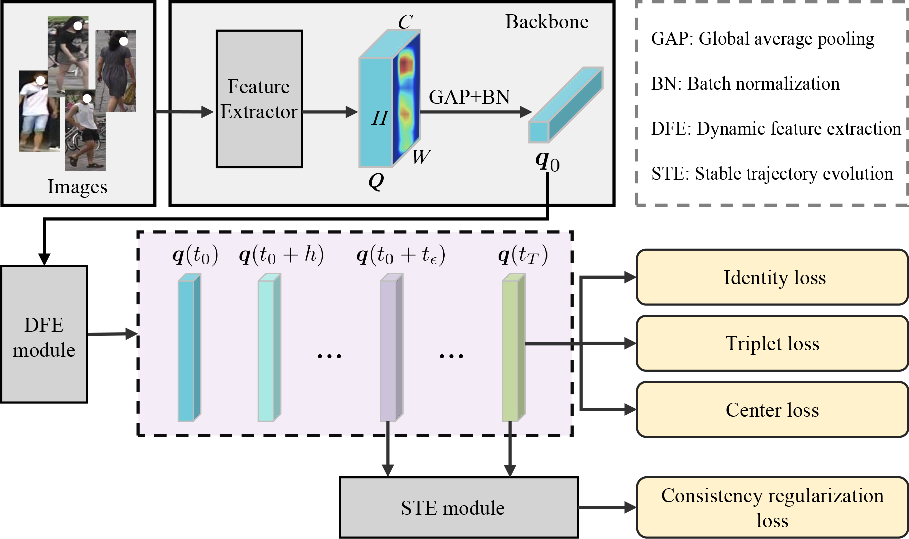
\includegraphics[width=4.0in]{Figure_1}
			\caption{\textcolor{yellow}{Schematic illustration of CODEN. It primarily consists of the backbone, the DFE module, and the STE module. In the backbone, we utilize a feature extractor to extract the person features. In the DFE module, we consider the features extracted by the backbone as the initial value in the dynamical system and further extract the global features. Based on the global features, the identity loss, triplet loss, and center loss are calculated. In the STE module, we input the global features and intermediate features to compute the consistency regularization loss.}}
			\label{fig:CODEN_framework}
		\end{figure*}
		
		\subsection{Dynamic feature extraction module}
		Due to factors such as camera viewpoints and human poses, identity-relevant information is often limited, while pedestrian images may include interference from identity-irrelevant information. For such cases, relying solely on the basic ResNet50 \cite{he2016deep} for learning features results in suboptimal discriminative performance and is prone to introducing interference factors. The non-intersecting property refers to integral curves originating from a point and is influenced by neighboring curves. Dynamical systems controlled by ODEs possess this non-intersecting property, making them more robust against adversarial attacks compared to convolutional neural networks \cite{chen2018neural, yan2019robustness}. Consequently, we introduce an ODE-controlled dynamical system into the person Re-ID task and design a DFE module to mitigate the impact of interfering factors and extract pedestrian saliency information. The core motivation of the DFE module is that features of pedestrians with the same identity are close to each other in the representation space. This module constrains the features along the integral curves of neighboring pedestrians with the same identity, thereby promoting identity feature learning.
		
		The DFE module primarily consists of an ODE block and an integrator. The ODE block is designed to establish a parameterized ODEs that describes the complex temporal evolution of pedestrian features. The input to the ODE block is the features $\boldsymbol{q}(t)$, and the output is the evolution function ${\mathrm{d}\boldsymbol{q}(t)}/{\mathrm{d}t}$ over time. The integrator dynamically solves these equations, extracting discriminative pedestrian features. It outputs the features at the next time step, $\boldsymbol{q}(t + h)$, where $h$ represents the step size. A schematic diagram of the DFE module architecture is shown in Fig. \ref{fig:ode_module}.
		
		\begin{figure}[!htbp]
			\centering
			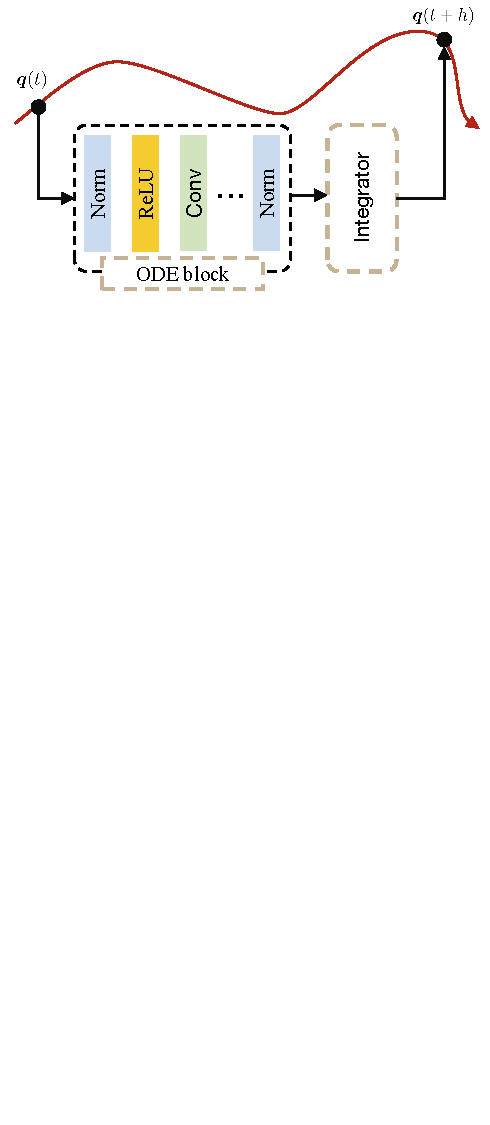
\includegraphics[width=2.5in]{Figure_2}
			\caption{Schematic illustration of DFE module. It primarily consists of an ODE block and an integrator. In the ODE block, we input the features from the previous time step and calculate the temporal evolution function of the dynamical system. In the integrator, we input the temporal evolution function to obtain the features for the next time step.}
			\label{fig:ode_module}
		\end{figure}
		
		In the ODE block, we formulate the ODE to describe the evolution of the features, as given by Eq. \eqref{eq:Node}:
		\begin{equation}
			\label{eq:Node}
			\left.\left\{\begin{array}{l}\frac{\mathrm{d}\boldsymbol{q}(t)}{\mathrm{d}t}=f_{\boldsymbol{\theta}}(t,\boldsymbol{q}(t)),\quad t\in[t_{0},t_{T}]\\\boldsymbol{q}(t_0)=\boldsymbol{q}_{0}\end{array}\right.\right.,
		\end{equation}
		where $t$ denotes the evolution time over the interval $[t_0, t_T]$, $\boldsymbol{q} \in \mathbb{R}^{d}$ represents the $d$-dimensional state of the differential equation, and $f_{\boldsymbol{\theta}}(\cdot)$ is a trainable function parameterized by weights $\boldsymbol{\theta}$, consisting primarily of $1\times1$ convolutional layers, group normalization layers, and ReLU activation functions.
		
		In the integrator, we employ the fourth-order Runge-Kutta (RK4) scheme to compute pedestrian features, as described by Eq. \eqref{eq:RK4_scheme}:
		\begin{equation}
			\label{eq:RK4_scheme}
			\boldsymbol q_{n+1}=\boldsymbol q_n+\frac{h}{6}\left(\boldsymbol k_1+2\boldsymbol k_2+2\boldsymbol k_3+\boldsymbol k_4\right),
		\end{equation}
		where
		\begin{equation}
			\begin{aligned}
				&\boldsymbol k_{1} =f_{\boldsymbol{\theta}} \left(t_n, \boldsymbol q_{n}\right), \\
				&\boldsymbol k_{2} =f_{\boldsymbol{\theta}} \left(t_n+\frac{h}{2}, \boldsymbol q_{n}+\frac{h}{2}\boldsymbol{k}_{1}\right), \\
				&\boldsymbol k_{3} =f_{\boldsymbol{\theta}} \left(t_n+\frac{h}{2}, \boldsymbol q_{n}+\frac{h}{2}\boldsymbol{k}_{2}\right), \\
				&\boldsymbol k_{4} =f_{\boldsymbol{\theta}} \left(t_n+h, \boldsymbol q_{n}+h\boldsymbol{k}_{3}\right),
			\end{aligned}
		\end{equation}
		where $h$ is the step size.
		
		\subsection{Stable trajectory evolution module}
		The shapes of pedestrians are often irregular, which makes random rectangular perturbation strategies likely to introduce ambiguities, potentially diminishing the benefits of adversarial representations. Therefore, the STE module utilizes features sampled along the system trajectories as perturbations to the initial value of the dynamical system, simulating the noisy information introduced by non-target pedestrians. It then employs a consistency regularization loss to control differences between the perturbed features and their non-perturbed counterparts, reducing the impact of irrelevant factors on Re-ID performance.
		
		Considering an intermediate time $t_0+t_{\epsilon} \in (t_0, t_T)$, the corresponding features $\boldsymbol{q}(t_0+t_{\epsilon} )$ can be expressed as:
		\begin{equation}
			\label{eq:ode_intermeidate}
			\begin{aligned}
				\boldsymbol{q}(t_0+t_{\epsilon} ) = \boldsymbol{q}(t_0) + \int_{t_0}^{t_0+t_{\epsilon}}f_{\boldsymbol{\theta}}(t, \boldsymbol q(t))\mathrm{d}t.
			\end{aligned}
		\end{equation}
		The features $\boldsymbol{q}(t_0+t_{\epsilon} )$ can be regarded as the result of perturbations applied to $\boldsymbol{q}(t_0)$. If $\boldsymbol{q}(t_0+t_{\epsilon} )$ is taken as the initial condition in Eq. \eqref{eq:Node}, the solution is $\boldsymbol{q}(t_T + t_{\epsilon})$. The difference between the perturbed features $\boldsymbol{q}(t_T+t_{\epsilon})$ and the non-perturbed features $\boldsymbol{q}(t_T)$ can be expressed as:
		\begin{equation}
			\label{eq:ode_gronwall_infer}
			\begin{aligned}
				\left\| \boldsymbol{q}(t_T+t_{\epsilon})-\boldsymbol q(t_T)\right\|_{2}=&\left\| \int_{t_T}^{t_T+t_{\epsilon}}f_{\boldsymbol{\theta}}(t, \boldsymbol q(t))\mathrm{d}t\right\|_{2}. \\
			\end{aligned}
		\end{equation}
		Applying the Gronwall-Bellman inequality, Eq. \eqref{eq:ode_gronwall_infer} can be reformulated as:
		\begin{equation}
			\label{eq:ode_gronwall_infer2}
			\begin{aligned}
				\left\| \boldsymbol{q}(t_T+t_{\epsilon})-\boldsymbol q(t_T)\right\|_{2}
				\leq&\left\|Se^{t_{\epsilon}}e^{\int_{t_T}^{t_T+t_{\epsilon}}\left|f_{\boldsymbol{\theta}}(t, \boldsymbol q(t))\right| \mathrm{d}t}\right\|_{2},
			\end{aligned}
		\end{equation}
		where $S>0$ represents a hyper-parameter used to adjust the difference between $\boldsymbol{q}(t_T+t_{\epsilon})$ and $\boldsymbol{q}(t_T)$. To minimize the difference, the consistency regularization loss is designed, as shown in Eq. \eqref{eq:steady_loss}:
		
		\begin{equation}
			\label{eq:steady_loss}
			\textcolor{yellow}{\mathcal{L}_{\text{con}}=\sum_{i=1}^{N}\left\|S e^{t_{\epsilon}}e^{\int_{t_T}^{t_T+t_{\epsilon}}\left|f_{\boldsymbol{\theta}}(t, \boldsymbol q_i(t))\right| \mathrm{d}t}\right\|_{2},}
		\end{equation}
		where $N$ represents the number of images. When $\mathcal{L}_{\text{s}}$ is sufficiently small, the model's outputs for each pedestrian with the same identity will stabilize around $\boldsymbol{q}(t_T)$.
		
		\subsection{Optimization}
		During the training phase, the identity loss $\mathcal{L}_{\text{id}}$, triplet loss $\mathcal{L}_{\text{tri}}$, center loss $\mathcal{L}_{\text{cen}}$, and consistency regularization loss $\mathcal{L}_{\text{con}}$ are used to optimize the network parameters. We adopt cross entropy loss as the identity loss to supervise feature learning, with label smoothing \cite{szegedy2016rethinking} employed to prevent overfitting. The identity loss $\mathcal{L}_{\text{id}}$ can be expressed as:
		\begin{equation}
			\mathcal{L}_{\text{id}}=-\sum_{k=1}^{N}\hat{y}_{k}\log s(\hat{p}_{k}),
		\end{equation}
		where $N$ denotes the number of images. The function $s(\cdot)$ signifies the softmax operation. $\hat{p}$ represents the predicted values generated by an identity classifier. The smoothed labels, denoted as $\hat{y}$, are computed with the $k$-th element calculated as follows:
		
		\begin{equation}
			\textcolor{yellow}{\hat{y}_k=(1-\epsilon_{y})y+\frac{\epsilon_y}{N},}
		\end{equation}
		where $0 < \epsilon_y < 1$ is the smoothing rate, typically set to 0.1, and $y$ denotes the sample labels.
		
		We employ triplet loss with hard sample mining \cite{luo2019bag}, which selects the farthest positive sample and the closest negative sample within a training batch to separate positive and negative samples by a certain margin. $P$ identities and $K$ images for each identity are randomly selected to form a batch of size $P \times K$. The triplet loss $\mathcal{L}_{\text{tri}}$ is defined as follows:
		
		\begin{equation}
			\mathcal{L}_{\text{tri}}=\sum_{i=1}^{PK}\left[\operatorname*{max}_{p\in\mathcal{P}}d_i^{a,p}-\operatorname*{min}_{n\in\mathcal{N}}d_i^{a,n}+m\right]_{+},
		\end{equation}
		where $m$ represents the margin between positive and negative sample pairs. $\left[x\right]_{+} = \max(x,0)$. $a$ is the index of the anchor image in the batch. $p$ and $n$ are the indices of the most challenging positive sample and the most challenging negative sample of index $a$ respectively. $\mathcal P$ and $\mathcal N$ represent the positive sample set and negative sample set of index $a$ respectively, that is, $\mathcal P =\left\{ p|y_p = y_a \right\}$ and $\mathcal N = \left\{ n|y_n \neq y_a\right\}$. $d$ denotes the Euclidean distance between feature representations.
		
		We adopt center loss \cite{wen2016discriminative}, which penalizes the distance between features and their corresponding class centers to encourage instances of the same class to be closer to their class center. Specifically, the loss $\mathcal{L}_{\text{cen}}$ is defined as follows:
		\begin{equation}
			\mathcal{L}_{\text{cen}}=\frac12\sum_{j=1}^{N}\left\| \boldsymbol q_{j}-\boldsymbol c_{y_{j}}\right\|_{2}^{2},
		\end{equation}
		where $y_{j}$ denotes the label of the $j$-th image, and $\boldsymbol{c}_{y_{j}}$ represents the learnable center of class $y_{j}$ in the feature space.
		
		Finally, the total loss $\mathcal{L}_{total}$ of our method during training is as follows:
		\begin{equation}
			\mathcal{L}_{total}=\lambda_{\text{id}}\mathcal{L}_{\text{id}} + \lambda_{\text{tri}} \mathcal{L}_{\text{tri}} + \lambda_{\text{cen}} \mathcal{L}_{\text {cen}}+ \lambda_{\text {con}} \mathcal{L}_{\text {con}},
		\end{equation}
		where $\lambda_{\text{id}}$, $\lambda_{\text{tri}}$, $\lambda_{\text{cen}}$, and $\lambda_{\text{con}}$ represent the weights assigned to the corresponding losses.
		
		\section{Experiment}	\label{section:experiment}
		In this section, we first detail the datasets used and the experimental settings. Next, we conduct an ablation study to examine the effectiveness of each module. Then, we evaluate the impact of hyper-parameters on the CODEN. Subsequently, the proposed method is compared with several existing methods. Finally, we provide a qualitative analysis of the experimental results.
		
		\subsection{Datasets and experimental settings}
		
		\textbf{Datasets.} We evaluate our method on three widely used Re-ID datasets, including Market-1501 \cite{zheng2015scalable}, DukeMTMC-reID \cite{ristani2016performance}, and CUHK03 \cite{zhong2017re}. The details of the datasets are provided in Table \ref{tab:dataset}.
		
		{Market-1501} dataset contains 32,668 images of 1,501 identities. All images are collected by 5 high-resolution and 1 low-resolution cameras deployed in the Tsinghua University campus. The train set consists of 12,936 images from 751 identities. The test set consists of 19,732 images from 750 identities.
		
		{DukeMTMC-reID} dataset contains 36,411 images of 1,404 identities from 8 cameras at Duke University. The train set consists of 16,522 images from 702 identities, and the test set consists of 19,889 images from 702 identities.
		
		{CUHK03} dataset contains images from 1,467 identities captured by 6 cameras at the Chinese University of Hong Kong. It is annotated into labeled and detected datasets. CUHK03-labeled dataset consists of 7,368 train images and 5,328 test images, while CUHK03-detected dataset consists of 7,365 train images and 5,332 test images. We partitioned the dataset according to the new protocol \cite{zhong2017re}, with 767 identities in the train set and the remaining 700 identities in the test set.
		
		\begin{table}[h]
			\caption{The detailed information of datasets. ID represents the number of identities. IMG represents the number of images.}
			\label{tab:dataset}
			\begin{tabular*}{\textwidth}{@{\extracolsep\fill}lccccc}
				\toprule
				& & \multicolumn{2}{@{}c@{}}{Train} & \multicolumn{2}{@{}c@{}}{Test}  \\
				\cmidrule{3-4}\cmidrule{5-6}%
				Dataset & Camera & ID & IMG & ID & IMG  \\
				\midrule
				Market-1501 & 6 & 751 & 12,936 & 750 & 19,732 \\
				DukeMTMC-reID & 8 & 702 & 16,522 & 702 & 17,661 \\
				CUHK03 & 6 & 767 & 7,368/7,365 & 700 & 5,328/5,332 \\
				\bottomrule
			\end{tabular*}
		\end{table}
		
		\textbf{Evaluation metrics.} Performance evaluation is conducted utilizing the cumulative matching curve (CMC) and mean average precision (mAP) metrics. The CMC protocol is used to evaluate the model's performance at Rank-$k$, where Rank-$k$ represents the expectation of finding the correct target at the $k$-th rank. The mAP protocol is used to evaluate the performance of multiple matching images in the gallery set. These metrics are jointly utilized for a comprehensive evaluation of the overall performance.
		
		\textbf{Implementation details.} The experiments are conducted on a machine equipped with an NVIDIA 3060 GPU, using the PyTorch framework. \textcolor{yellow}{During the data preprocessing phase, all images are resized to $256\times128$ pixels. In addition, a variety of data augmentation techniques are applied to enhance the diversity of the training data. These include random horizontal flipping, random cropping, padding, and random erasing.} Each batch comprises 60 images, with 4 identities per batch, and each identity includes 15 images. The dimension of the pedestrian features is set to 2,048. The weight hyper-parameters for the model are configured as follows: $\lambda_{\text{id}} = 1$, $\lambda_{\text{tri}} = 1$, $\lambda_{\text{cen}} = 5 \times 10^{-4}$, and $\lambda_{\text{con}} = 0.35$. The stable hyper-parameter is set to $S = 0.15$. For the numerical integration of the ODEs, the initial time is set  to $t_0 = 0$, the final time to $t_T = 0.04$, and the intermediate time to $t_\epsilon = 0.01$, the step size to $h = 0.01$. The training process employs the Adam optimizer for model parameter updates over 180 epochs. The initial learning rate is set to $3.5 \times 10^{-4}$ and decays by a factor of 0.1 after training for 40 and 70 epochs. The re-ranking technique is not employed for fair comparison.
		
		\subsection{Ablation studies}
		To evaluate the contribution of each module in the proposed CODEN, a series of ablation experiments were conducted by progressively adding or removing modules. ResNet50 \cite{he2016deep} was used as the baseline model. The results of these experiments are presented in Table \ref{tab:ablation}.
		
		\begin{table}[h]
			\caption{Ablation studies of the CODEN on the Market-1501 and DukeMTMC-reID datasets.}
			\label{tab:ablation}
			\begin{tabular*}{\textwidth}{@{\extracolsep\fill}lcccccc}
				\toprule%
				& \multicolumn{3}{@{}c@{}}{Market-1501} & \multicolumn{3}{@{}c@{}}{DukeMTMC-reID}  \\
				\cmidrule{2-4}\cmidrule{5-7}%
				Method  & mAP & R-1  & R-5  & mAP & R-1 & R-5   \\
				\midrule
				Baseline & 85.9  & 94.4  & 98.1  & 76.5  & 87.0  & 94.2  \\
				ODEN & 87.4  & 95.2  & 98.4  & 78.9  & 88.9  & 95.0  \\
				CODEN & \textbf{88.0} & \textbf{95.4}  & \textbf{98.6}  & \textbf{79.1}  & \textbf{89.6}  & \textbf{95.2} \\
				\bottomrule
			\end{tabular*}
		\end{table}
		
		\textbf{Effectiveness of the DFE module.} The effectiveness of the DFE module was investigated. ODEN integrates the DFE module into the baseline. Compared to the baseline, ODEN exhibits an improvement in mAP by 2.1\% and in \text{Rank-1} by 1.0\% on the Market-1501, and an improvement in mAP by 2.6\% and in Rank-1 by 2.4\% on the DukeMTMC-reID. These results demonstrate that the DFE module significantly enhances performance by combining feature learning with a dynamical system.
		
		\textbf{Effectiveness of the STE module.} The effectiveness of the STE module was investigated. The CODEN integrates both the DFE and STE modules. Compared to ODEN, CODEN shows improvements in mAP from 87.4\% to 88.0\% and in Rank-1 from 95.2\% to 95.4\% on Market-1501, and improvements in mAP from 78.9\% to 79.1\% and in Rank-1 from 88.9\% to 89.6\% on DukeMTMC-reID. The STE module reduces identity-irrelevant information interference by introducing feature perturbations and employing consistency regularization loss, which helps form a more discriminative feature space and enhances the robustness of recognition tasks.
		
		\textbf{Impact of the ODE block structrue.} The impact of the ODE block structure with different numbers of convolutional layers in CODEN on performance was investigated, with results presented in Table \ref{tab:ODE_level}. The optimal performance of CODEN is achieved with two convolutional layers. Deviations from this number, whether by increasing or decreasing the layers, result in a slight decrease in accuracy. This suggests that overly simplistic dynamic models may not capture essential pedestrian features, while excessively complex models could introduce unnecessary complications in network weight optimization. Therefore, maintaining a moderate number of layers in dynamic models is crucial for ensuring optimal performance.
		
		\begin{table}[h]
			\caption{Impact of ODE block structure for CODEN on the Market-1501 and DukeMTMC-reID datasets.}
			\label{tab:ODE_level}
			\begin{tabular*}{\textwidth}{@{\extracolsep\fill}lcccccc}
				\toprule%
				& \multicolumn{3}{@{}c@{}}{Market-1501} & \multicolumn{3}{@{}c@{}}{DukeMTMC-reID}  \\
				\cmidrule{2-4}\cmidrule{5-7}%
				Number of layers  & mAP & R-1  & R-5  & mAP & R-1 & R-5   \\
				\midrule
				1  & \textbf{88.1}  & 95.0  & 98.5  & 79.0  & 89.1  & 95.0  \\
				2  & 88.0  & \textbf{95.4}  & \textbf{98.6}  & \textbf{79.1}  & \textbf{89.6}  & 95.2  \\
				3  & 87.7  & 95.3  & 98.4  & 79.0  & 88.8  & \textbf{95.3}  \\
				4  & 87.6  & 95.3  & 98.3  & 78.9  & 88.8  & 95.0 \\
				\bottomrule
			\end{tabular*}
		\end{table}
		
		\textbf{Impact of the integral scheme.} The impact of the integral scheme has been investigated. We compared the impact of the Euler scheme, the Midpoint scheme, and the RK4 scheme on the Market-1501 dataset. The experimental results are presented in Table \ref{tab:integral_scheme}. Compared to the Euler scheme, the RK4 scheme improves mAP and Rank-1 accuracy by 0.4\% and 0.3\%, respectively. When compared to the Midpoint scheme, it enhances mAP and Rank-1 accuracy by 0.3\% and 0.1\%, respectively. These results indicate that while the RK4 scheme is more computationally intensive, it offers more accurate and stable recognition. Therefore, the appropriate integral scheme can be selected based on the specific requirements for accuracy and efficiency in different scenarios.
		
		\begin{table}[h]
			\caption{Impact of different integral schemes for CODEN on the Market-1501 dataset. Error represents the accumulated error of the scheme. $t_{\text{train}}$ represents the training time for each iteration.}
			\label{tab:integral_scheme}
			\begin{tabular*}{\textwidth}{@{\extracolsep\fill}lcccccc}
				\toprule%
				Scheme & Error & $t_{\text{train}}$ & mAP & R-1  & R-5  & R-10 \\
				\midrule
				Euler  & $\mathcal{O}(h)$  & 0.35 s/it  & 87.6  &95.0 & 98.5 & 99.1  \\
				Midpoint  & $\mathcal{O}(h^2)$  & 0.36 s/it & 87.7  & 95.3 & 98.5 & 99.1    \\
				RK4  & $\mathcal{O}(h^4)$  & 0.39 s/it &  88.0  &95.4 &98.6  & 99.1    \\
				\bottomrule
			\end{tabular*}
		\end{table}
		
		\textbf{Cross-dataset evaluation.} The generalization ability of a method is a crucial factor in its suitability for practical deployment. To evaluate the CODEN's generalization capability, we conducted a cross-dataset evaluation for recognizing unseen pedestrians and scenes. Models trained on one dataset are evaluated on a different dataset. The experimental results are presented in Table \ref{tab:Generalization_Ability_Analysis}. Compared to the baseline, CODEN achieves improvements of 8.9\% in mAP and 9.5\% in Rank-1 from Market-1501 to DukeMTMC-reID, and 6.0\% in mAP and 7.4\% in Rank-1 from DukeMTMC-reID to Market-1501. This indicates that the design of the DFE and STE modules is effective, and CODEN enhances the ability to effectively recognize unseen pedestrians as well as scenes.
		
		\begin{table}[h]
			\caption{Cross-domain evaluation on Market-1501 and DukeMTMC-reID datasets. Market $\rightarrow$ DukeMTMC represents that the model is trained on source domain Market-1501 and tested on target domain DukeMTMC-reID, and vice versa.}
			\label{tab:Generalization_Ability_Analysis}
			\begin{tabular*}{\textwidth}{@{\extracolsep\fill}lcccccc}
				\toprule%
				& \multicolumn{3}{@{}c@{}}{Market $\rightarrow$ Duke} & \multicolumn{3}{@{}c@{}}{Duke $\rightarrow$ Market}  \\
				\cmidrule{2-4}\cmidrule{5-7}%
				Method  & mAP & R-1  & R-5  & mAP & R-1 & R-5   \\
				\midrule
				Baseline & 17.9  & 32.2  & 47.2  & 21.5  & 47.9  & 63.2  \\
				ODEN & 25.7  & 40.9  & 56.6  & 26.3  & 53.3  & 69.2  \\
				CODEN & \textbf{26.8}  & \textbf{41.7} & \textbf{58.0}  & \textbf{27.5}  & \textbf{55.3} & \textbf{71.4} \\
				\bottomrule
			\end{tabular*}
		\end{table}
		
		\subsection{Parameter analysis}
		The CODEN introduces two crucial training hyper-parameters: $\lambda_{\text {con}}$  and $S$. In order to investigate the impact of these parameters on performance, numerous experiments were conducted on the Market-1501 dataset, and the results are illustrated in Fig. \ref{fig:parameter_analysis}.
		
		\begin{figure}[!htbp]
			\centering
			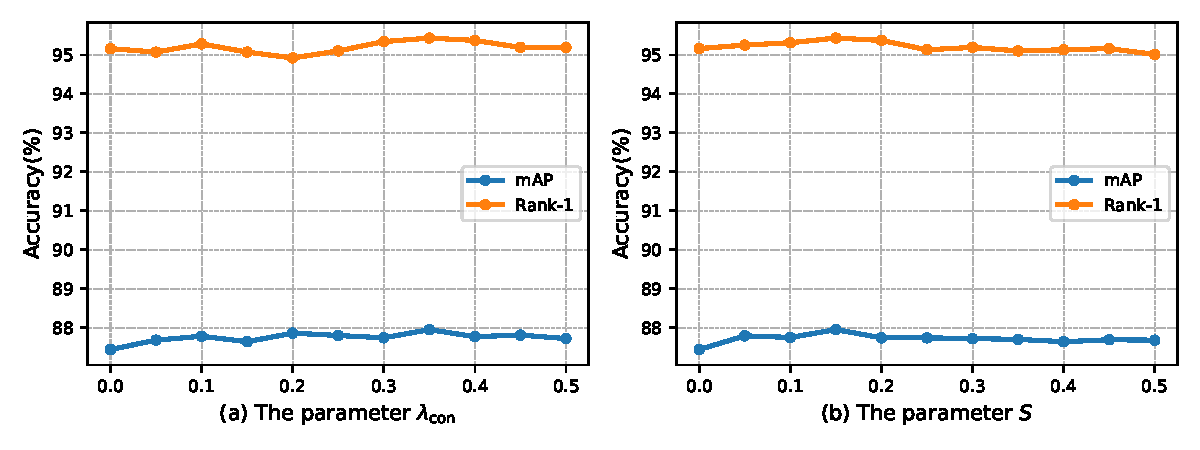
\includegraphics[width=5in]{Figure_3}
			\caption{Analysis of parameters: (a) the impact of the parameter $\lambda_{\text {con}}$ and (b) the impact of the parameter $S$}
			\label{fig:parameter_analysis}
		\end{figure}
		
		\textbf{Impact of parameter  $\lambda_{\text {con}}$.} The parameter $\lambda_{\text {con}}$ affects the strength of supervision on global feature stability. We set $\lambda_{\text {con}}$ within the range of 0 to 0.5, and the results are illustrated in Fig. \ref{fig:parameter_analysis}(a). As the value of $\lambda_{\text {con}}$ increases, both mAP and rank-1 show an upward trend. CODEN achieves peak performance when $\lambda_{\text {con}} = 0.35$. However, with further increases in $\lambda_{\text {con}}$, performance declines, possibly due to an excessive emphasis on stability, which compromises the model’s discriminative properties. These results indicate that both insufficient and excessive supervision of global feature stability lead to a decline in performance.
		
		\textbf{Impact of parameter $S$.} The parameter $S$ is a factor influencing the difference between integral curves. We set $S$ within the range of 0 to 0.5, and the results are depicted in Fig. \ref{fig:parameter_analysis}(b). When the value of the parameter $S$ is small, the dynamic trajectories propagated forward by the ODEs may rapidly change near the termination time. This behavior increases the rigidity of the dynamical system and reduces recognition performance. Conversely, when the value of the parameter $S$ is large, pedestrian features may aggregate irrelevant information, making it difficult to learn distinctive information. At $S=0.15$, both the mAP and Rank-1 reach their peaks. The results further validate the effectiveness of the consistency regularization loss.
		
		\subsection{Performance comparison}
		To ensure a fair evaluation of CODEN's performance, we compared it against several existing methods on the Market-1501, DukeMTMC-reID, and CUHK03 datasets. The comparison results are presented in Table \ref{tab:STOA}. CODEN shows competitive performance in these benchmark datasets.
		
		\begin{table}[h]
			\caption{Comparing with the state-of-the-art methods on the Market-1501, DukeMTMC-reID, and CUHK03 datasets.}
			\label{tab:STOA}
			\begin{tabular*}{\textwidth}{@{\extracolsep\fill}lcccccccc}
				\toprule%
				& \multicolumn{2}{@{}c@{}}{Market-1501} & \multicolumn{2}{@{}c@{}}{DukeMTMC-reID} & \multicolumn{2}{@{}c@{}}{CUHK03-detected} & \multicolumn{2}{@{}c@{}}{CUHK03-labeled} \\
				\cmidrule{2-3}\cmidrule{4-5}\cmidrule{6-7}\cmidrule{8-9}
				Method & mAP & R-1 & mAP & R-1 & mAP & R-1 & mAP & R-1 \\
				\midrule
				PCB \cite{sun2018beyond} & 77.4  & 92.3  & 65.3  & 81.9  & - & - & 54.2  & 61.3  \\
				PCB+RPP \cite{sun2018beyond} & 81.6  & 93.8  & 69.2  & 83.3  & - & - & 57.5  & 63.7  \\
				HA-CNN \cite{li2018harmonious} & 75.7  & 91.2  & 63.8  & 80.5  & 41.0  & 44.4  & 38.6  & 41.7  \\
				MLFN \cite{chang2018multi} & 74.3  & 90.0  & 62.8  & 81.0  & 49.2  & 54.7  & 47.8  & 52.8  \\
				MGCAM \cite{song2018mask} & 74.3  & 83.6  & - & - & 49.9  & 49.3  & 46.8  & 46.3  \\
				BOT \cite{luo2019bag} & 85.9  & 94.5  & 76.4  & 86.4  & 62.7   & 65.6 & 65.0  & 66.5  \\
				PGR  \cite{li2019pose} & 77.2  & 93.9  & 66.0  & 82.6  & - & - & - & - \\
				P$^2$-Net \cite{guo2019beyond} &  83.4 & 94.0  & 70.8  & 84.9 & 64.2 & 71.6 &  69.2 & 75.8 \\
				PGFA \cite{miao2019pose} & 81.4  & 94.6  & 72.7  & 85.7  & - & - & - & - \\
				FPO \cite{tang2020person} & 79.2  & 91.8  & - & - & 56.3  & 63.1  & 60.2  & 65.6  \\
				IGOAS \cite{zhao2021incremental} & 84.1 & 93.4 & 75.1 & 86.9 & - & - & - & - \\
				AFELN \cite{zhang2021appearance} & 81.3  & 93.3  & 72.9  & 86.5  & - & - & 61.7  & 66.5  \\
				AND \cite{ghorbel2022masking} & 87.8  & 92.3  & 63.7  & 83.8  & 56.5  & 60.6  & 55.6  & 61.9  \\
				ICAMFL \cite{wang2023information} & 82.3  & 93.3  & 71.6  & 85.6  & 59.3  & 64.6  & 63.3  & 67.1  \\
				PRE-Net \cite{yan2023part} &86.5 &95.3 & 77.8 & 89.3 &  - & - & - & - \\
				SRFnet \cite{tian2023self} & 85.7 & 94.2 & 77.9 & 89.1 &69.6 & 73.3 &72.4 &75.0 \\
				ETNDNet \cite{dong2023erasing} & 87.2 & 95.3 & 77.9 & 88.5 &  - & - & - & - \\
				\textbf{CODEN} & \textbf{88.0}  & \textbf{95.4}  & \textbf{79.1}  & \textbf{89.6}  & \textbf{70.2} & \textbf{73.6} & \textbf{73.0} & \textbf{76.5} \\
				\bottomrule
			\end{tabular*}
		\end{table}
		
		On the Market-1501 dataset, CODEN achieves an impressive mAP of 88.0\% and Rank-1 of 95.4\%. Compared to the defense-based method ETNDNet  \cite{dong2023erasing}, CODEN shows improvements of 0.8\% in mAP and 0.1\% in Rank-1. Compared to the local-based method PCB+RPP \cite{sun2018beyond}, CODEN shows improvements of 6.4\% in mAP and 1.6\% in Rank-1. Additionally, CODEN demonstrates competitive advantages compared over other methods.
		
		On the DukeMTMC-reID dataset, the proposed CODEN achieves a mAP of 79.1\% and Rank-1 of 89.6\%. Compared to the global-based method BOT \cite{luo2019bag}, CODEN exhibits improvements of 2.7\% and 3.2\% in mAP and Rank-1, respectively. Compared to the cues-based method PGFA \cite{miao2019pose}, CODEN shows improvements of 6.4\% in mAP and 3.9\% in Rank-1. CODEN outperforms other methods, achieving better performance on both evaluation metrics.
		
		On the CUHK03 dataset, the proposed CODEN achieves a mAP of 70.2\% and Rank-1 of 73.6\% on the automatically detected data, and a mAP of 73.0\% and Rank-1 of 76.5\% on the manually labeled data. Compared to the global-based method ICAMFL \cite{wang2023information}, CODEN shows improvements of 10.9\% in mAP and 9.0\% in Rank-1 on the detected data, and 9.7\% in mAP and 9.4\% in Rank-1 on the labeled data. Compared with other methods, CODEN shows significant performance advantages. These results demonstrate the effectiveness of CODEN.
		
		\subsection{Qualitative analysis}
		To qualitatively validate the effectiveness of CODEN, we conducted a visualization analysis of saliency. Saliency maps are generated by extracting the maximum values along the channel dimension of features, enabling an intuitive understanding of the focus on different regions. Red regions exhibit higher attention, while blue regions display lower attention. Fig. \ref{fig:vis_heatmap} presents the visualization results, clearly illustrating the superiority of CODEN over the baseline. The baseline shows localized hotspots, which are susceptible to interference and can potentially lead to erroneous identification results. CODEN exhibits multiple highly activated hotspots. This enables a more precise perception of pedestrian details and the extraction of as many relationships and regional features as possible. It showcases its outstanding performance in feature representation and recognition. This further validates the effectiveness and superiority of CODEN in the task of person Re-ID.
		
		\begin{figure}[!htbp]
			\centering
			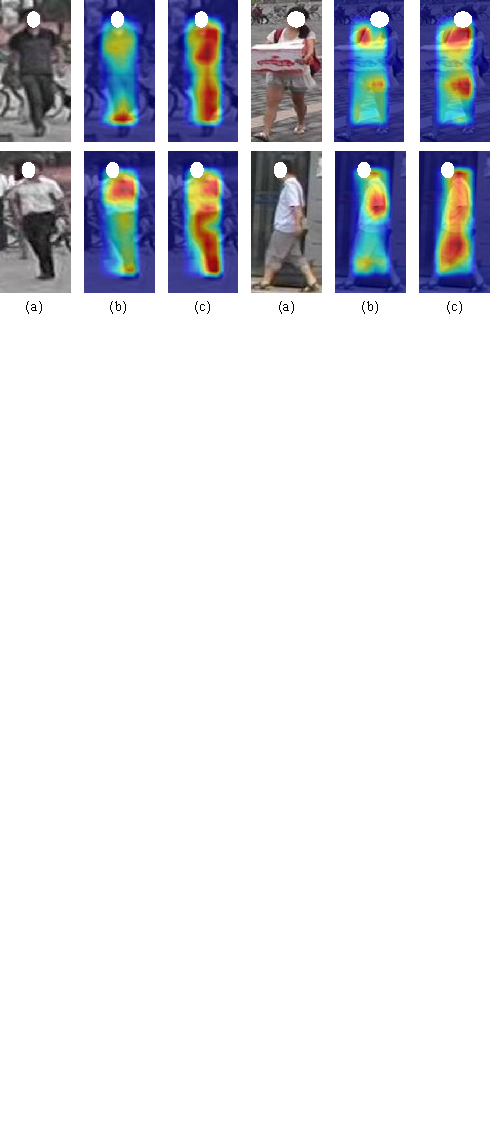
\includegraphics[width=9cm]{Figure_4}
			\caption{Visualization of regions of interest by the method. (a) Original image. (b) Heatmap generated by the baseline. (c) Heatmap generated by CODEN.}
			\label{fig:vis_heatmap}
		\end{figure}
		
		\section{Conclusion}
		\label{section:conclusion}
		Person Re-ID is an important research field with huge application potential and challenges. In this paper, we present the CODEN for Re-ID, which establishes a nonlinear dynamic model using ODEs to better mine pedestrian information. By introducing feature perturbation and incorporating a consistency regularization loss, CODEN effectively regularizes system trajectories, thereby reducing the influence of identity-irrelevant information. Despite the proposed method has achieved  progress on the two evaluation metrics, there is still room for further improvement. For example, the impact of different forms of dynamic models on recognition performance deserves further study.
		
		% \disclosures
		\subsection*{Disclosures}
		The authors declare no conflict of interest.
		
		\subsection* {Code, Data, and Materials Availability}
		The codes and datasets generated and/or analyzed during the current study are available from the corresponding author on reasonable request.
		
		
		\subsection* {Acknowledgments}
		This study has been supported by the National Natural Science Foundations of China under Grant Nos. 12172186, 11772166.
		
		
		%%%%% References %%%%%
		
		\bibliography{report}   % bibliography data in report.bib
		\bibliographystyle{spiejour}   % makes bibtex use spiejour.bst
		
		%%%%% Biographies of authors %%%%%
		
		\vspace{2ex}\noindent\textbf{Yin Huang} was born in 1995. He is currently a PhD candidate at the College of Computer Science and Technology, Qingdao University, China. He received his Master's degree from Liaoning University of Technology, China, in 2021. His research interest is multi-body dynamics and computer vision.
		
		\vspace{2ex}\noindent\textbf{Jieyu Ding}  is currently a professor at the School of Mathematics and Statistics, and the Center for Computational Mechanics and Engineering Simulation of Qingdao University, China. She received her PhD degree in Shanghai University, and Shanghai Institute of Applied Mathematics and Mechanics, China, in 2008. Her research interest includes multi-body system dynamics, design optimization, and optimal control.
		
		\listoffigures
		\listoftables
		
	\end{spacing}
\end{document}